%% This is file FCEFyN-paper.tex is the template file for publications
%% in the "Revista de la Facultad de Ciencias Exactas, Físicas y Naturales
%% de la Universidad Nacional de Córdoba, Argentina,
%% https://revistas.unc.edu.ar/index.php/FCEFyN.
%% This file was originally written by Gustavo J. Krause.
%% First revision: 2018-07-17
%% Second revision: 2018-07-26 by Mariano Lizarraga (minor modifications)
%%
%% History:
%%           2018-07-20  First version by Gustavo Krause
%%

% Opciones específicas:
%     esp:   Idioma español (por defecto)
%     eng:   Idioma inglés
%     por:   Idioma portugués
%     blind: Se compila la versión para revisores (se ocultan datos de los autores)


\documentclass[esp]{FCEFyN-class}
%
% Título de la publicación
\title{Instrucciones para autores de la Revista de la Facultad de Ciencias
       Exactas, Físicas y Naturales}

% Título corto para el encabezado (copiar el título principal si no resulta demasiado largo)
\shorttitle{Instrucciones para autores de la Revista de la FCEFyN}
       
% Autores
\author[1]{Nombre A. Apellido}
\author[2]{Nombre B. Apellido}
\author[1,2,3]{Nombre C. Apellido}

% Afiliaciones de los autores
\affil[1]{Nombre de Departamento o Instituto,
Nombre Universidad, Provincia o Estado, País}
\affil[2]{(Otro) Nombre de Departamento o Instituto,
Nombre Universidad, Provincia o Estado, País}
\affil[3]{(Otro) Nombre de Departamento o Instituto,
Nombre Universidad, Provincia o Estado, País}

% Apellido del primer autor del trabajo
\firstauthor{Apellido}

% Datos del autor de contacto
\contactauthor{Nombre A. Apellido}           % Nombre y apellido del autor de contacto
\email{nombre.apellido@email.com}            % Correo electrónico del autor de contacto
\mailingaddress{Dirección postal completa}   % Dirección postal completa
\phonenumber{1234-5678 int. 123}             % Número de teléfono

% Datos de la publicación (serán definidas en la edición)
\thisvolume{XX}
\thisnumber{XX}
\thismonth{MES}
\thisyear{20XX}
\receptiondate{dd/mm/aaaa}
\acceptancedate{dd/mm/aaaa}
\publicationdate{dd/mm/aaaa}


% Coloque aquí sus definiciones particulares
\newcommand{\vect}[1]{\mathbf{#1}}  % vectores


% Iniciar documento
\begin{document}

% Introduzca aquí el resumen en español (o en portugués si utiliza la opción [por])
\resumen{
Este documento brinda una plantilla para la preparación de trabajos originales que desean ser
publicados en la Revista de la Facultad de Ciencias Exactas, Físicas y Naturales de la Universidad
Nacional de Córdoba, Argentina.
Se recomienda que el resumen contenga entre 150 y 200 palabras en un solo párrafo, donde deben
resumirse el contexto, la motivación, la metodología empleada, los aportes más originales, los
resultados y las conclusiones de su trabajo.
No deben incluirse citas bibliográficas y se recomienda no introducir acrónimos ni fórmulas en el
resumen o en el título. No haga referencias a figuras o a tablas. Como recomendación general, escriba
su artículo insertando y eliminado texto a partir de este documento. De esta forma, le será más fácil
respetar los estilos predefinidos.}

% Introduzca aquí las palabras clave en español (o en portugués si utiliza la opción [por])
\palabrasclave{
Primera palabra o frase clave, segunda palabra o frase clave, tercera palabra o frase clave. 
(Coloque entre tres y seis palabras o frases clave separadas por coma, las cuales representan la
temática de su trabajo)}

% Insert here the abstract in English language
\abstract{
Write in English the same text inserted in the ``resumen''.}

% Insert here the keywords of your work in English language
\keywords{
Translate to English the same words and phrases written above.}

% Incluir título, autores, resumen, etc.
\maketitle
\thispagestyle{fancy}
\printcontactdata

% Cuerpo principal del trabajo
\section{Introducción}
\primerapalabra{L}{a}% Letra capital en primera palabra
Revista de la Facultad de Ciencias Exactas, Físicas y Naturales es el órgano oficial de publicación
de esta Institución, la cual pertenece a la Universidad Nacional de Córdoba, Argentina. Su objetivo es 
difundir trabajos originales que contribuyan al desarrollo de las distintas áreas de la ciencia y la
tecnología. La misma se publica en formato electrónico con una frecuencia semestral. Se aceptarán
para su publicación artículos originales, revisiones y comentarios bibliográficos, comunicaciones
breves, notas técnicas e historias de casos sobre temas específicos que cubran las diversas áreas de
interés involucradas en las carreras que se dictan en la Facultad de Ciencias Exactas, Físicas y
Naturales (Ingenierías en sus diferentes especialidades, Biología y Geología).

Los idiomas aceptados son español, inglés y portugués. Para ajustar la plantilla a cada uno de ellos,
utilice las opciones \texttt{esp} (opción por defecto), \texttt{eng} o \texttt{por}, respectivamente.
Los artículos deberán tener una extensión máxima de diez mil palabras, en tanto que las comunicaciones
breves y las revisiones bibliográficas no podrán superar las dos mil palabras.

El formato sobre el que se basó este documento es el utilizado por el IEEE para la mayoría de sus
publicaciones y conferencias. Sin embargo, se han realizado algunos cambios, como por ejemplo, en el
presente estilo se utiliza formato A4 y los márgenes se han fijado en 2 cm a la izquierda y arriba, y
1,5 cm a la derecha y abajo.
El ancho de columna en se ha fijado en 8,5 cm, con una separación de 0,5 cm entre ellas. Además,
se ha dejado un encabezado de página indicando el código del artículo (el cual será completado en el 
proceso final de edición y publicación). En el pie de página se incluye sólo el número de página.

Las definiciones elementales de estilo son: fuente Times o Times New Roman para todas las partes del
documento, tamaño 20 pt para el título, 12 pt para los autores, 9 pt y cursiva para la línea de la
institución a la que pertenecen los autores, 9 pt para el resumen y palabras clave, 10 pt para el
texto normal, ecuaciones y 12 pt versales para títulos de sección, 11 pt versales para el título de 
nivel 1, itálica para los títulos de nivel 2 y 3, 9 pt para los epígrafes de las figuras, tablas y
referencias (todas estas definiciones ya están fijadas en el archivo de clase provisto).
Utilice \emph{cursivas} para destacar un término (no subrayado). A pesar de todos estos
detalles y cuantos otros que se podrían dar, se recomienda nuevamente escribir su artículo copiando,
pegando y reemplazando texto a partir de este mismo documento. Esta es la forma más fácil y segura de
respetar los estilos definidos. Por favor, no redefina ningún elemento del estilo (tipografía,
espacios entre textos, márgenes, u otras medidas definidas en el archivo de clase).

La estructura general que se espera para este artículo abarca secciones como: introducción,
materiales, métodos, resultados, discusión, conclusiones, trabajos futuros, agradecimientos y 
referencias. Estos títulos pueden combinarse de a dos en una misma sección y los títulos trabajos 
futuros y agradecimientos son totalmente optativos. Es común que la sección de métodos lleve otro 
título más relacionado con el aporte original del artículo, pero las restantes secciones se presentan
con los títulos antes listados. Si existieran demostraciones u otros desarrollos matemáticos extensos,
se recomienda agruparlos en apéndices antes de las referencias bibliográficas.

A continuación se darán más detalles acerca de las secciones del documento y los formatos para 
insertar los distintos tipos de objetos, como ecuaciones, figuras y tablas.


\section{Formatos para los objetos insertados}
En el formato de esta publicación las secciones y subsecciones del documento no se numeran y 
se insertan con los comandos tradicionales de \LaTeX, es decir
\begin{verbatim}
  \section{Nombre sección}
  \subsection{Nombre subsección}
  \subsubsection{Nombre subsubsección}
\end{verbatim}
El formato para los párrafos ya incluye una sangría 
automática en la primera línea y un espacio extra para la separación entre párrafos.

\subsection{Las ecuaciones}
Las ecuaciones menores o definiciones de variables pueden insertarse directamente en la línea del
párrafo, por ejemplo, considérese que se desea definir una historia $\vect{h}_i^n = w_{i-1}. w_{i-2},
\dots, w_{i-n+1}$ asociada a un símbolo $w_i$. Observe que una manera sencilla de asegurar la 
uniformidad en el estilo de las ecuaciones es escribir las formulaciones matemáticas siempre en el
entorno correspondiente, es decir, utilizando \verb!$a + b$! para escribir por ejemplo $a + b$
(no escribir directamente como el texto a + b). Por otro lado, recuerde que las unidades de medición
deben escribirse siempre en formato \emph{redonda}, de modo que éstas no se confundan con variables
(por ejemplo, debe escribirse $1\,\text{m} = 100\,\text{cm}$ en lugar de $1m = 100cm$).

Para insertar ecuaciones más complejas o que deban ser referenciadas, se recomienda utilizar los
entornos de ecuaciones disponibles en el paquete \verb!amsmath!, recordando que la orden 
\verb!\begin{equation}! numera automáticamente las ecuaciones. Para escribir ecuaciones sin
numeración utilice \verb!\begin{equation*}! o simplemente \verb!$$<expresión>$$! para
obtener la expresión en una línea aparte, por ejemplo $$ \frac{a + b + c}{2} = d. $$
En el caso de una ecuación numerada, se debe definir su \emph{etiqueta} con el comando
\verb!\label{ec-1}!:
%----- Ecuación.
\begin{equation} \label{ec-1}
 P_l(w_i|\vect{h}_i^{k}) = \sum_{j=0}^{k-1} \lambda_j \hat{P}(w_i|\vect{h}_i^{j}).
\end{equation}
%----- Fin. Ecuación.
Para hacer referencia a esta ecuación desde el texto debe utilizarse el comando \verb!\eqref{ec-1!,
el cual coloca automáticamente el número de la ecuación entre paréntesis. Por ejemplo, ``en
ec.~\eqref{ec-1} se puede ver la estimación de la probabilidad de una historia a partir de la simple
combinación lineal de historias de orden inferior''.
Recuerde que el uso de \emph{entrecomillados} en \LaTeX debe realizarse utilizando los comandos
correspondientes, es decir mediante \verb!``texto''! para obtener ``texto''.

Si su trabajo implica la utilización de formulaciones matemáticas extensas como en la
ec.~\eqref{ec-2}, las cuales no pueden visualizarse correctamente en el formato de dos columnas,
puede emplear un flotante extendido con el comando \verb!\begin{figure*}[! para disponer la ecuación
en el ancho total de la página y en la parte superior del texto.
Recuerde utilizar correctamente los delimitadores $(\mbox)$, $[\mbox]$, $\{\mbox\}$ a través de los
comandos \verb!\left* \right*! para que su tamaño se ajuste automáticamente a la expresión matemática.
%----- Ecuación dos columnas.
\begin{figure*}[!t]
 \begin{equation}\label{ec-2}
   b = \left\{\frac{1}{\alpha_1 + 1}\left(x_s - x_i\right)^{\alpha_1+1} + \frac{k}{\alpha_2 + 1}
   \left[\left(c - x_i\right)^{\alpha_2+1} - \left(x_s - x_i\right)^{\alpha_2+1}\right]
   + \frac{\beta}{\beta + 1}\left[\left(x_s - x_i\right)^{\alpha_1} - 
   \left(x_s + x_i\right)^{\alpha_2}\right]\right\}^{-1}.
 \end{equation}
\end{figure*}
%----- Fin. Ecuación dos columnas.


\subsection{Las figuras}
Las figuras deben incluirse debidamente referenciadas utilizando los comandos de \LaTeX tradicionales,
y nunca deben colocarse como elementos sueltos dentro del texto.
El pie o epígrafe de figura se coloca automáticamente utilizando el entorno
\begin{verbatim}
\begin{figure}[!tb]
  \centering
  \includegraphics[<options>]{<file>}
  \caption{Epígrafe} \label{<etiqueta>}
\end{figure}
\end{verbatim}
y rellenando el campo correspondiente en \verb!\caption{<>}! (ver Fig.~\ref{fig-1}). Las figuras pueden contenerse en archivos PDF, JPG o PNG, entre otros. Dentro del campo \verb![<options>]! se puede utilizar el modificador
\verb![width=.8\columnwidth]! si es necesario ajustar el tamaño de la figura, como ejemplo se ha fijado el
factor \verb!.8!.

%----- Figura.
\begin{figure}[!tb] 
 \centering
 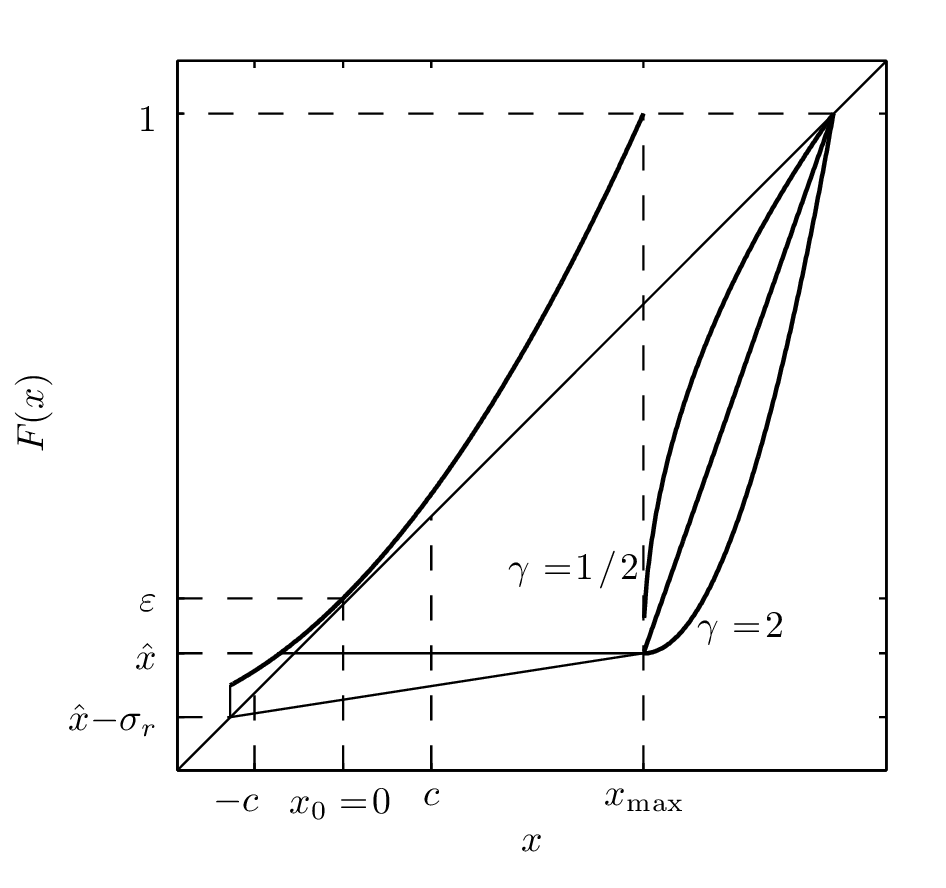
\includegraphics[width=.8\columnwidth]{figura1} 
 \caption{Esquema del mapa utilizado indicando las diferentes formas de reinyección y el efecto
          del ruido.} \label{fig-1}
\end{figure}
%----- Fin. Figura.

Preferentemente, las figuras deben disponerse al comienzo o al final de una columna de texto (para lo
cual se hace uso de la opción \texttt{[!tb]}), y en general no es recomendable disponer las figuras en
páginas especiales al final del trabajo.
No incluya saltos ni espacios adicionales en los extremos de las figuras ya que éstos se encuentran
debidamente definidos en el archivo de clase.
Si en la figura se utilizan ejes cartesianos, recuerde siempre describir a qué corresponde cada
eje (etiquetas) con una fuente de tamaño no menor a 7 pt para facilitar la lectura.
Para hacer referencia a una figura se debe utilizar la forma abreviada Fig. seguida
del comando \verb!\ref{etiqueta}!, salvo cuando esté al comienzo de un párrafo, caso en que se
deberá utilizar la palabra completa.

%----- Figura dos columnas.
\begin{figure*}[!tb] 
 \centering
 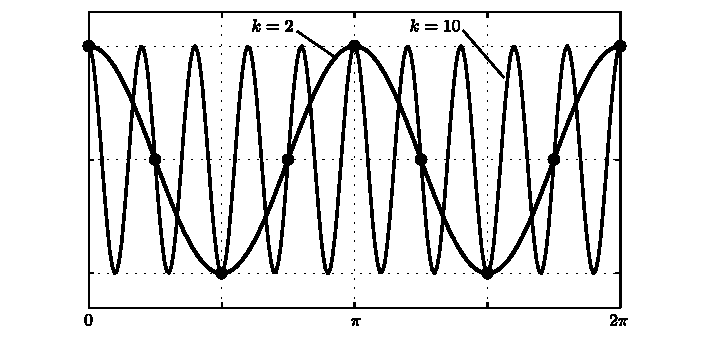
\includegraphics{figura2.pdf} 
 \caption{Ejemplo del \emph{aliasing} que se produce en una grilla con $N = 8$ nodos. Ambos modos
          ($k = 2$ y $k = 10$) toman los mismos valores en los puntos de la grilla.} \label{fig-2}
\end{figure*}
%----- Fin. Figura dos columnas.

En lo posible, no incluya colores en las gráficas, preferentemente utilice distintos tipos de líneas.
Además, tenga en cuenta que los gráficos vectorizados brindan una mejor calidad electrónica y de
impresión, por lo tanto, inserte todas las gráficas con algún formato vectorizado o bien, si se
tratase de una fotografía o imagen más compleja, utilice formatos con compresión sin pérdida de
información (se pueden configurar los formatos JPG, PNG, TIF,GIF, etc).
Para incluir figuras que requieran ser visualizadas en el ancho total de la página debe utilizarse
nuevamente el entorno \verb!\begin{figure*}!, como en el caso de la Fig.~\ref{fig-2}.


\subsection{Las tablas}
Es preferible que las tablas se diseñen utilizando los comandos de \LaTeX definidos para tal efecto,
y no que se inserten como archivos de imágenes ya que esto va en detrimento de la calidad del
documento. Sin embargo, esta opción puede resultar aceptable si la inserción se hace a partir de un
formato vectorizado que respete el tamaño y el estilo de la tipografía.
El epígrafe de las tablas es marcadamente diferente al pie de las figuras. En este caso se coloca por
arriba de la tabla, con fuente de tamaño 8 pt y párrafo centrado.
Al igual que en las figuras, es preferible que las tablas se encuentren al principio o al pie de una
columna. El tamaño del texto dentro de las tablas no debería ser inferior a 7 pt ni mayor a 10 pt (el
tamaño de letra utilizado en el texto general).
Un ejemplo de este estilo puede verse en la Tabla~\ref{tabla-1}.

\begin{table}[!b]
 \centering
  \caption{Resultados finales y reducción relativa de los errores (promedios sobre 10 particiones de
 entrenamiento y prueba).} \label{tabla-1}
 {\small
 \begin{tabular}{ccccc}
  \hline
  \hline
  \thead{Errores de \\ reconocimiento} & \thead{SER \\ \%} & \thead{WER \\ \%} & \thead{WAER \\ \%} &
                        \thead{Reducción \\ \% WER} \\
  \hline
  \hline
  Referencia & $38.30$ & $7.54$ & $8.53$ & $-$ \\
  \hline
  HMM-PASS & $30.55$ & $5.36$ & $6.67$ & $28.91$ \\
  1-PASS & $25.50$ & $4.76$ & $5.70$ & $36.87$   \\
  \hline
  \hline
 \end{tabular}}
\end{table}

\subsection{Las citas bibliográficas}
Las citas bibliográficas se realizarán en el sistema Harvard, el cual utiiza el formato
\emph{(Autor/es,~año)} para indicar la referencias dentro del texto, separando con comas los autores e
incorporando la expresión \emph{et~al.}, disponiendo todo entre paréntesis. Por ejemplo, para un autor
\citep{Alarcos1999}, dos autores \citep{ArslanHansen1996} y tres o más autores \citep{WangEtAl2015}.
Para esta tarea, la plantilla utiliza \texttt{Bibtex} y el paquete \texttt{natbib}, con lo cual las
referencias deben ser incluidas en un archivo \texttt{*.bib} externo (\texttt{Referencias.bib} en este
ejemplo).
De esta manera, la referencia a una cita bibliográfica se hace con el comando
\verb!\citep{<etiqueta>}!, y la inclusión textual de una cita se hace por medio de
\verb!\citet{<etiqueta>}!, para obtener por ejemplo: ``como se observa en el libro de
\citet{Mitchell2001}''.

En el acápite de la Bibliografía el estilo para los diferentes tipos de citas bibliográficas
consiste en:
\begin{itemize}
 \item Libro: Autor/es, año entre paréntesis. Título en cursiva, editorial, lugar de publicación
 \citep{Alarcos1999}. Se incluye mediante la opción \texttt{@book} en el archivo de referencias.
%
 \item Capítulo de libro: Autor/es, año entre paréntesis. Título del capítulo entre comillas.
 En: título del libro en cursiva del libro, páginas, editorial, lugar de publicación
 \citep{Mitchell2001}. Se incluye con el campo \texttt{@inbook} en el archivo de referencias.
%
 \item Artículo en revista periódica: Autor/es, año entre paréntesis. Título del artículo entre
 comillas, nombre de la revista en cursiva, volumen, número entre paréntesis, páginas
 \citep{ArslanHansen1996,WangEtAl2015}. Se incluye mediante la opción \texttt{@article}.
%
 \item Conferencias y simposios: Autor/es, año entre paréntesis. Título del artículo entre comillas.
 En: título de las memorias o del evento en cursiva, editorial de la publicación de las memorias,
 lugar de publicación, páginas \citep{BarkovaJouvet1999}. Se incluye con el campo
 \texttt{@inproceedings} en el archivo de referencias.
%
 \item Sitio Web: Autor/es, año entre paréntesis. Título del artículo entre comillas, tomado de
 <URL>, fecha de consulta de la página web entre paréntesis \citep{CFDwebpage}. Se incluye con la
 opción \texttt{@webpage}.
%
 \item Reporte técnico: Autor/es, año entre paréntesis. Título del reporte entre comillas,
 ``Reporte Nº'', institución en cursiva, lugar de publicación \citep{NACA460}. Se incluye
 mediante el campo \texttt{@techreport}.
%
 \item Tesis, tesina o trabajo final: Autor/es, año entre paréntesis. Título en cursiva, tipo de
 trabajo. Institución, lugar de presentación \citep{Krause2014}. Se incluye utilizando el campo
 \texttt{@thesis} en el archivo de referencias.
%
 \item Manual o memoria técnica: Autor/es, año entre paréntesis. Título en cursiva, organización o
 institución, lugar de publicación \citep{Indura2010}. Se incluye con la opción \texttt{@manual}.
%
 \item Otrass formas de comunicación: para referenciar otras formas de comunicación siempre debe
 especificar el autor o entidad, el año y la manera en que fue realizada la comunicación.
 Opcionalmente puede incluir un título y una nota aclaratoria \citep{Radio2015}. Este tipo de 
 referencias se incluyen utilizando el campo \texttt{@other}.
\end{itemize}

La sección de referencias bibliográficas se titula como ``Referencias'' (o con su equivalente
dependiendo del idioma elegido) y posee un estilo particular para el párrafo, donde se elimina la
sangría y se reduce el tamaño de fuente (se fija en 8 pt).
Las referencias deben presentarse en orden alfabético teniendo en cuenta el apellido del primer autor,
independientemente del orden de aparición en el texto. Recuerde que todas las referencias incluidas en
la bibliografía deben estar debidamente citadas en el texto.

Para satisfacer completamente las definiciones establecidas para la bibliografía y facilitar las
tareas posteriores de edición y publicación, se recomienda enfáticamente utilizar el estilo de
referencias provisto (\texttt{FCEFyN-refs-esp.bst} o del idioma correspondiente), incluyendo la
bibliografía mediante el comando
\begin{verbatim}
 \insertbibliography{<archivo.bib>} 
\end{verbatim}
al final del trabajo.

\subsection{Otras recomendaciones generales}
Defina adecuadamente cada uno de los acrónimos empleados describiendo su significado la primera vez
que aparecen en el texto. Por ejemplo, ``dicha relación se conoce como relación de grandes masas
(RGM)''. Una vez definido, utilice siempre el acrónimo en lugar del término completo.
Recuerde definir cada uno de los símbolos que aparecen en las expresiones matemáticas y no olvide
aclarar la notación empleada cuando se utilicen operadores matemáticos especiales o poco comunes.
La utilización de mayúsculas debe hacerse de acuerdo a las convenciones generales, es decir,
al comienzo de una oración luego de un punto, en nombres propios, en acrónimos, etc., y en los títulos
de acuerdo a lo definido en el formato del trabajo.
Ante cualquier duda comunicarse a revista@efn.uncor.edu.


\section{Conclusiones}
En las conclusiones se deberá presentar una revisión de los puntos clave del artículo con especial
énfasis en el análisis y discusión de los resultados que se realizó en las secciones anteriores y en
las aplicaciones o ampliaciones de éstos. No debe reproducir el resumen en esta sección ni repetir
párrafos ya incluidos en otras secciones del trabajo.


\section{Agradecimientos}
En el caso de que existan agradecimientos, referencias a proyectos de investigación, o entidades 
financiadoras del trabajo, éstos deben incluirse en la sección de ``Agradecimientos'' luego de las
conclusiones del trabajo.
Verifique colocar correctamente los nombres y/o códigos correspondientes a los proyectos de
investigación, instituciones, programas de financiamiento, etc., involucrados en el trabajo.

% Incluir apéndices (si fuera necesario)
\appendix
\section{Apéndices}
En algunas situaciones conviene incluir una sección de apéndices con sus correspondientes subsecciones.

\subsection{Demostraciones}
Pueden incluirse demostraciones dentro del texto principal siempre que la la extensión de las mismas 
y su complejidad no distraigan al lector de los contenidos más relevantes del trabajo. En caso
contrario, se recomienda disponer en el texto solamente los resultados finales incluyendo las
demostraciones en un apéndice al final del trabajo.

\subsection{Algoritmos}
Del mismo modo que en el caso anterior, siempre que los algoritmos no sean demasiado extensos pueden
incluirse dentro del cuerpo principal del trabajo, de lo contrario deberán disponerse en un apéndice
al final del trabajo.

\subsection{Otros datos}
La inclusión de detalles técnicos, mediciones accesorias, tablas de datos u otro tipo de información
relevante para el trabajo debe hacerse en forma de apéndice cuando su extensión lo justifique, de lo
contrario pueden incluirse directamente en el cuerpo principal del texto cuando se hace referencia a
los mismos.

% Incluir las referencias
\insertbibliography{Referencias.bib}

\end{document}
